D\section{Ekran startowy aplikacji i przygotowanie danych}
Kiedy dane zostały dostosowane do działania systemu, można przystąpić do implementacji pozostałych części rozwiązania.
Kolejnym elementem jest ekran startowy aplikacji, widoczny na rysunku \ref{fig:homescreen}. Zawiera on przyciski, które przekierowują użytkownika do odpowiednich sekcji aplikacji.

\begin{figure}[h]
    \centering
    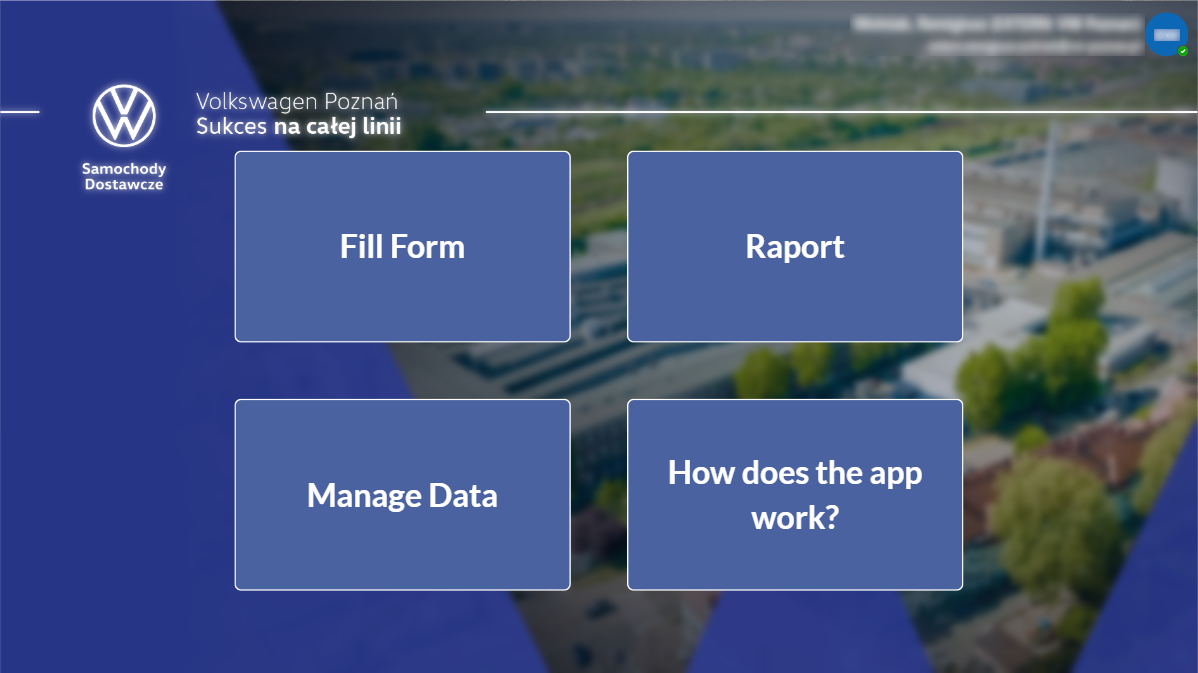
\includegraphics[width=0.9\textwidth]{figures/HomeScreen.png}
    \caption{Ekran startowy aplikacji} 
    \label{fig:homescreen}
\end{figure}

Dodatkowo, podczas uruchomienia aplikacji, pobierane są dane z list SharePointowych a następnie odpowiednio przetwarzane w celu płynnego wyświetlania ich w aplikacji. \\
Kod w języku \emph{Power Fx} wywoływany podczas uruchamiania aplikacji został przedstawiony na listingu \ref{lst:OnStartCode}.

\lstset{language=C,caption={Kod wywoływany podczas uruchamiania aplikacji},label=lst:OnStartCode}
\begin{lstlisting}[language=PowerFx]
 Set(varDownloadingData;true);;
 ClearCollect(colYears;{Value: Text(Now();"yyyy")-2};
 {Value: Text(Now();"yyyy")-1};
 {Value: Text(Now();"yyyy")+0};
 {Value: Text(Now();"yyyy")+1};
 {Value: Text(Now();"yyyy")+2}
 );;
 
 ClearCollect(colNumbers; {Value: 1};{Value: 2};{Value: 3};{Value: 4};{Value: 5});;
 
 Set(UserVar;UżytkownicyusługiOffice365.MyProfile());;
 
 // W OnStart aplikacji lub OnVisible ekranu
 ClearCollect(LocalServiceData; Lista_Uslug);;
 ClearCollect(LocalCostData; Lista_Kwot);;
 ClearCollect(LocalIndicationsData; Lista_Indykacji);;
 ClearCollect(
     MergedData;
     AddColumns(
         Lista_Uslug;
         Kwoty; LookUp(
             Lista_Kwot;
             Service_ID = Lista_Uslug[@Service_ID] &&
             Year = Max(Filter(Lista_Kwot; Service_ID = Lista_Uslug[@Service_ID]); Year)
         );
         Indykacje; LookUp(
             Lista_Indykacji;
             Service_ID = Lista_Uslug[@Service_ID] &&
             Year = Max(Filter(Lista_Indykacji; Service_ID = Lista_Uslug[@Service_ID]); Year) &&
             IndicationNo = Max(Filter(Lista_Indykacji; Service_ID = Lista_Uslug[@Service_ID] && Year = Max(Filter(Lista_Indykacji; Service_ID = Lista_Uslug[@Service_ID]); Year)); IndicationNo)
         )
     )
 );;
 Set(varDownloadingData;false);;
 \end{lstlisting}

 W pierwszej kolejności funkcja \emph{Set}, przypisuje zmiennej \textit{varDownloadingData} wartość \textit{true}.
 Odpowiada ona za wyświetlenie indykatora ładowania oraz zablokowanie elementów ekranu co ma na celu zabezpieczenie przed wprowadzaniem zmian podczas ładowania się aplikacji.
Następnie wywołana zostaje funkcja \emph{ClearCollect}, która tworzy kolekcję o nazwie \textit{colYears}, przekazanej jako pierwszy argument. Drugi argument zawiera tablicę, która ma być przypisana do kolekcji. Zawiera ona pięc elementów, które są rokami wykorzystywanymi w polach \emph{Dropdown}.
W podobny sposób powstaje kolekcja \textit{colNumbers}, która zawiera numery indykacji.
Funkcja \emph{Set} w linii 12, pobiera informacje dotyczące obecnego użytkownika. 
Później powstają lokalne kopie trzech list: \textit{LocalServiceData}, \textit{LocalCostData} oraz \textit{LocalIndicationsData}.

Przedostatnim krokiem jest utworzenie kolekcji \textit{MergedData}, która zawiera połączone informacje z list \textit{Lista\_Uslug}, \textit{Lista\_Kwot} oraz \textit{Lista\_Indykacji}.
Funcja \emph{AddColumns()} jako pierwszy argument przyjmuje nazwy kolumn, drugi, opcjonalny argument to źródło z którego pobierane są dane natomiast trzecim jest warunekiem określającym jakie kolumny ze źródła wyodrębnić. Dodawane kolumny wyszukiwane są w innych listach z użyciem funkcji \emph{LookUp()} oraz \emph{Filter()}.
Kolekcja ta łączy ze sobą dane dopasowując je  względem \emph{Service\_ID}, \emph{Year} oraz \emph{IndicationNo} tworząc tabelę zawierającą informacje z najnowszej indykacji.

Na końcu do zmiennej \textit{varDownloadingData} przypisywana jest wartość \textit{false}, co oznacza, że dane zostały już pobrane i aplikacja jest gotowa do użytku.

Celem pobrania lokalnych kopii list, jest przyspieszenie działania mechanizmu filtrowania podczas wyboru usługi do edycji. 



